% BlinkTwin manuscript, IEEE two-column journal format (IEEEtran). Build: latexmk -pdf main.tex
% Supplementary material: supplement.tex (same build).
\documentclass[journal]{IEEEtran}
\usepackage[T1]{fontenc}
\usepackage{amsmath,amssymb}
\usepackage{graphicx}
\usepackage{booktabs}
\usepackage{array}
\usepackage{multirow}
\usepackage{xcolor}
\usepackage{cite}
\usepackage{url}
\usepackage[hidelinks]{hyperref}
\graphicspath{{figures/}{../results/}{../docs/img/}}
\newcolumntype{L}[1]{>{\raggedright\arraybackslash}p{#1}}
\newcommand{\KSS}{\mathrm{KSS}}
\newcommand{\RT}{\mathrm{RT}}
\hyphenation{Blink-Twin Media-Pipe Kal-man drow-si-ness}
% Draft placeholders (removed when filled)
\providecommand{\SIMABSTRACT}{\textbf{[simulation result]}}
\providecommand{\POWERTEXT}{\textbf{[power]}}
\providecommand{\SIMSECTION}{\textbf{[simulation]}}
\providecommand{\DISCUSSION}{\textbf{[discussion]}}
\providecommand{\SIMFORECAST}{\textbf{[forecast results]}}

\begin{document}

\title{BlinkTwin: Questionnaire-Anchored Estimation and Forecasting of Subjective Sleepiness From Webcam and Reaction-Time Signals in a Web Browser}

\author{Utsav~Poudel%
\thanks{U. Poudel is an independent researcher, Kathmandu, Nepal (e-mail: utsav.poudel@outlook.com.au).}%
\thanks{Code, analysis scripts and aggregate results: \url{https://github.com/r11up/BlinkTwin}.}}

\markboth{Manuscript submitted for review}{Poudel: BlinkTwin}

\maketitle

\begin{abstract}
\emph{Objective:} To estimate and forecast subjective sleepiness on an ordinary laptop by combining a biomathematical model, occasional self-ratings and passive signals, and to test the approach on public data.
\emph{Methods:} BlinkTwin runs in a web browser; video never leaves the page. A Kalman filter tracks the person's offset from the Three-Process Model of alertness, updated by Karolinska Sleepiness Scale (KSS) check-ins. A 3-min psychomotor vigilance test, blink duration and PERCLOS enter through forward models fitted within person on DROZY (14 adults), each with its own personal anchor state. We replayed the released model on DROZY leaving one subject out, ran its webcam pipeline on DROZY video against the electro-oculogram (EOG), analysed OpenNeuro ds004902 (33 adults), and ran a simulation with misspecified scenarios.
\emph{Results:} On DROZY, the mean absolute error of predicted KSS was 1.73 points for the prior, 1.51 with one check-in, 1.47 with passive signals and 1.38 with all three; intervals overlapped and a protocol-aware baseline gave 1.39. Webcam blink rates agreed with EOG (Spearman $\rho = 0.71$) and blink duration tracked KSS within person ($r = 0.58$), but PERCLOS failed on near-infrared video. On ds004902, offsets persisted weakly ($r = 0.29$) and a field-refitted KSS mapping lowered the prior's error from 1.69 to 1.46. In simulation, anchored fusion lowered the error of check-ins alone by 0.03 points; fusion without anchors failed.
\emph{Conclusion:} Check-ins set the level; passive signals can be added safely only with their own anchors, and their gains were small.
\emph{Significance:} An open, on-device implementation and a pre-specified protocol for testing personal sleepiness models in daily life.
\end{abstract}

\begin{IEEEkeywords}
Digital twin, Kalman filter, Karolinska Sleepiness Scale, PERCLOS, psychomotor vigilance test, sleepiness, Three-Process Model, webcam.
\end{IEEEkeywords}

\section{Introduction}
\label{sec:intro}

\IEEEPARstart{S}{leep} loss impairs performance in ways that matter for safety. In a classic comparison, 17~h of sustained wakefulness reduced performance on a tracking task to the level seen at a blood alcohol concentration of 0.05\%, and 24~h to the level seen at 0.10\%~\cite{dawson1997fatigue}. People are also poor judges of the impairment that builds up over days of short sleep: under chronic sleep restriction, lapses on the psychomotor vigilance test (PVT) keep increasing while sleepiness ratings level off~\cite{vandongen2003cumulative}, and individual differences in subjective and objective vulnerability to sleep loss are stable but unrelated~\cite{leproult2003individual}.

Three kinds of tool address parts of this problem. \emph{Biomathematical fatigue models} predict sleepiness or performance from the sleep--wake history and the time of day~\cite{borbely1982two,akerstedt1997three,akerstedt2004predictions,hursh2004fatigue,mallis2004summary,dawson2011modelling}. They need no sensor, and some of them are individualised from repeated performance tests~\cite{olofsen2004nonlinear,vandongen2007optimization,rajaraman2008individualized,liu2017real,reifman2019twobalert}. \emph{Ocular measures} such as PERCLOS and blink duration track drowsiness~\cite{wierwille1994research,dinges1998evaluation,caffier2003experimental,schleicher2008blinks}, and blinks can be detected in ordinary video~\cite{soukupova2016real}, but most systems map them to drowsiness with one rule for everyone, although the link between eyelid signs and sleepiness differs between people~\cite{ingre2006subjective}. \emph{Validated questionnaires}, such as the Karolinska Sleepiness Scale (KSS)~\cite{akerstedt1990subjective}, capture how sleepy a person feels and track performance and EEG changes~\cite{kaida2006validation,akerstedt2014subjective}, but they can be asked only a few times a day.

This paper asks whether an ordinary laptop can combine all three: keep a continuously updated estimate of how sleepy a person feels, state its uncertainty, and project it forward, with video kept on the device. We call the result a personal digital twin in the sense of a person-specific model that is updated from that person's data and can be queried for forecasts and what-if scenarios~\cite{grieves2017digital,corralacero2020digital}. The model itself is a small state-space model, and we use that term in the technical sections.

The difficulty lies in combining sources that disagree. A webcam or reaction-time signal can read a particular person consistently high or low. If such a signal is averaged with the person's ratings, it pulls the estimate away from what the person reports. BlinkTwin therefore gives each passive signal a forward measurement model with its own personal \emph{anchor}: a slowly drifting bias state, in the signal's own units, that absorbs where this person's signal sits relative to the population. Check-ins set the level of the estimate, and passive signals contribute mainly through their changes. Bias states in a Kalman filter are a standard technique~\cite{friedland1969treatment}; the contribution here is to apply them to self-rated sleepiness and to test the result.

Because the KSS is the reference, BlinkTwin estimates \emph{subjective} sleepiness. Given the dissociation described above, the application also shows the latest reaction test read on the population scale, and it flags a possible gap only when the person's own reaction times slow over a day or a week while their ratings do not.

The short answer from public data and simulation is that check-ins and the biomathematical prior do most of the work. Passive signals add a little, and only when the model estimates each person's bias in each signal; a filter that merely allows for those biases gains nothing. The website's camera pipeline measures blinks on laboratory video but not PERCLOS, and the passive signals' benefit has yet to be shown in real use. We report these limits alongside the method because they decide what the planned study has to test.

\paragraph*{Contributions}
\begin{enumerate}
  \item An open, on-device implementation that joins the published Three-Process Model of alertness~\cite{akerstedt2004predictions,akerstedt2008accounting,ingre2014validating} with KSS check-ins and forward models of a 3-min PVT (PVT-B), blink duration and PERCLOS in one Kalman filter, with a personal anchor for each passive signal (Sections~\ref{sec:system} and~\ref{sec:model}).
  \item An evaluation on public data: a leave-one-subject-out replay of the model on DROZY~\cite{massoz2016ulg}; a test of the website's camera pipeline on DROZY's near-infrared video against the electro-oculogram (EOG), which exposed a failure of PERCLOS that we then guarded against; and tests of the offset premise and of the prior on OpenNeuro ds004902~\cite{xiang2024resting} (Section~\ref{sec:realdata}).
  \item A simulation study, reported following Morris et al.~\cite{morris2019using}, with a consider-covariance comparator~\cite{schmidt1966application}, a known-parameter reference, scenarios that break the model's assumptions, and a sensitivity analysis of the filter settings (Section~\ref{sec:simulation}).
  \item A planned protocol for a prospective validation study, to be registered before data collection (Section~\ref{sec:protocol}).
\end{enumerate}

BlinkTwin is a self-monitoring and research tool for desk work. It is not a medical device, it must not be used to decide whether someone is fit to drive or operate machinery, and the absence of an alert does not indicate alertness.

\section{Related work}
\label{sec:related}

\paragraph{Subjective scales.} The KSS asks people to rate their sleepiness over the last few minutes on a 9-point scale from ``extremely alert'' to ``very sleepy, great effort to keep awake, fighting sleep'' \citep{akerstedt1990subjective}. KSS ratings rise with time awake and at night and are associated with slower reaction times and EEG markers of sleepiness \citep{kaida2006validation}. The Stanford Sleepiness Scale (SSS) is an older 7-point alternative \citep{hoddes1973quantification}. For workload, NASA-TLX rates mental, physical and temporal demand, performance, effort and frustration on 0--100 scales; the unweighted mean (raw TLX) is widely used \citep{hart1988development,hart2006nasa}. Subjective ratings are one of several ways to measure cognitive load, alongside performance and physiological measures \citep{paas2003cognitive}.

\paragraph{Psychomotor vigilance.} The psychomotor vigilance test (PVT) measures simple reaction time to a stimulus that appears at random intervals \citep{dinges1985microcomputer}. It is sensitive to sleep loss, and lapses and response speed are its most sensitive outcomes \citep{basner2011maximizing}. The 3-minute PVT-B uses inter-stimulus intervals of 1--4~s and a lapse threshold of 355~ms, and it detects total and partial sleep deprivation \citep{basner2011validity}.

\paragraph{Eyelid and blink measures.} PERCLOS, the proportion of time the eyelids are at least 80\% closed, was found to track PVT lapses and was recommended for drowsiness monitoring \citep{wierwille1994evaluation,dinges1998perclos}. Blink duration and the lid-closing and reopening times increase with sleepiness \citep{caffier2003experimental,schleicher2008blinks}, and blink rate has been studied as a fatigue marker \citep{stern1994blink}. The size of these effects differs between people \citep{ingre2006subjective}.

\paragraph{Blink detection from video.} The eye aspect ratio (EAR), computed from six landmarks around each eye, detects blinks in ordinary video \citep{soukupova2016real}. MediaPipe provides real-time face meshes on consumer devices \citep{kartynnik2019real,lugaresi2019mediapipe}; its Face Landmarker also returns blendshape coefficients, including one for the closure of each eye. Public drowsiness datasets include DROZY \citep{massoz2016ulg} and the UTA Real-Life Drowsiness Dataset \citep{ghoddoosian2019realistic}.

\paragraph{Biomathematical models and individualisation.} The two-process model combines a homeostatic sleep pressure that builds during waking with a circadian rhythm \citep{borbely1982two}. The Three-Process Model of alertness adds sleep inertia and maps the result onto the KSS \citep{akerstedt1997three,akerstedt2004predictions}. Bayesian individualisation of the two-process model from repeated PVT data improves performance prediction during sleep deprivation \citep{rajaraman2008individualized}, and a mobile application brings this to real-time use \citep{reifman2019twobalert}. BlinkTwin differs in three ways: it targets the person's own subjective sleepiness and workload rather than PVT performance; it adds passive webcam signals between tests; and it models a separate bias for each passive channel so that the person's ratings stay the reference.

\paragraph{Digital twins of people.} The digital twin idea came from engineering \citep{grieves2017digital} and has been proposed for precision medicine, for example in cardiology \citep{corralacero2020digital}. A twin of a person's moment-to-moment state is a smaller target: it needs a model of how the state evolves, measurements that update it, and a way to ask what would happen under a different choice.

\begin{table}[t]
  \centering
  \caption{BlinkTwin compared with categories of prior work. Entries describe what is typical of each category in the cited work; individual systems vary. $\checkmark$: yes; $\times$: no; $\sim$: partly or varies.}
  \label{tab:comparison}
  \small
  \begin{tabular}{@{}L{6.2cm}ccccc@{}}
    \toprule
    & Live & Personal & Forecast, & Uncer- & On-device, \\
    Category & sensing & calibration & what-if & tainty & open \\
    \midrule
    Biomathematical models (two-process, Three-Process, SAFTE) \citep{borbely1982two,akerstedt1997three,hursh2004fatigue} & $\times$ & $\times$ & $\checkmark$ & $\times$ & $\sim$ \\
    Individualised models from repeated PVTs (2B-Alert) \citep{rajaraman2008individualized,reifman2019twobalert} & $\sim$ & $\checkmark$ & $\checkmark$ & $\sim$ & $\sim$ \\
    Camera drowsiness detectors (PERCLOS, blinks) \citep{dinges1998perclos,soukupova2016real} & $\checkmark$ & $\times$ & $\times$ & $\times$ & $\sim$ \\
    PVT tests and apps \citep{dinges1985microcomputer,basner2011validity} & $\sim$ & $\times$ & $\times$ & $\times$ & $\sim$ \\
    Questionnaires (KSS, NASA-TLX) \citep{akerstedt1990subjective,hart1988development} & $\times$ & $\times$ & $\times$ & $\times$ & $\checkmark$ \\
    \midrule
    \textbf{BlinkTwin} (this work) & $\checkmark$ & $\checkmark$ & $\checkmark$ & $\checkmark$ & $\checkmark$ \\
    \bottomrule
  \end{tabular}
\end{table}

\section{System}
\label{sec:system}

\begin{figure}[t]
  \centering
  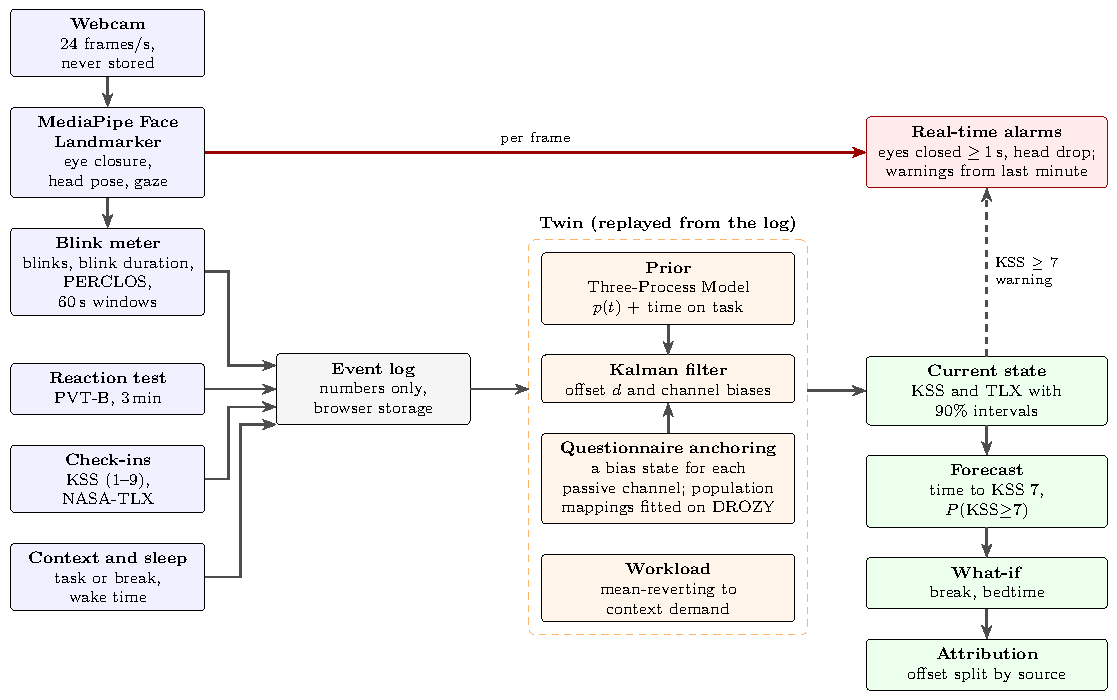
\includegraphics[width=\linewidth]{figures/architecture.pdf}
  \caption{BlinkTwin architecture. Webcam frames are processed in the page and discarded. Per frame, eye closure and head pose drive real-time alarms. Per minute, a summary of the eyes is stored as an event, together with reaction-test results, check-ins and context entries. The twin's state at any time is rebuilt by replaying these events through one Kalman filter.}
  \label{fig:architecture}
\end{figure}

BlinkTwin is a single-page web application written in TypeScript (Figure~\ref{fig:architecture}). It needs a laptop with a webcam and a current browser, and nothing is installed. All computation runs in the page.

\subsection{Webcam sensing}
Frames from the webcam are passed, at up to 24 per second, to the MediaPipe Face Landmarker \citep{kartynnik2019real,lugaresi2019mediapipe} in video mode, with one face, blendshapes and the facial transformation matrix enabled. For each frame the eye-closure score $c_t$ is the mean of the \texttt{eyeBlinkLeft} and \texttt{eyeBlinkRight} blendshapes (0 = open, 1 = closed), or missing when no face is found.

The open-eye level of this score differs between people, cameras and lighting, so the \emph{blink meter} normalises it against the person's own recent baseline. With $b_t$ the 20th percentile of $c$ over the previous 30~s,
\begin{equation}
  \hat c_t = \min\!\left(1, \max\!\left(0, \frac{c_t - b_t}{1 - b_t}\right)\right).
\end{equation}
A closure starts when $\hat c_t \geq 0.5$ and ends when $\hat c_t \leq 0.3$ (hysteresis). Closures lasting 50--1000~ms are counted as blinks; longer ones are counted separately as long closures. Every 60~s the meter reports the blink rate, the mean blink duration, the number of long closures, PERCLOS (the fraction of frames with a face in which $\hat c_t \geq 0.8$) and coverage (the fraction of frames with a face). These per-minute windows are the only camera data that are stored. The same blink meter, unchanged, was run on landmark data from DROZY and validated against the electro-oculogram (Section~\ref{sec:grounding}).

\paragraph{Head pose and gaze.} Pitch, yaw and roll are computed from MediaPipe's facial transformation matrix and expressed relative to the person's resting pose, the median of the last 20~s. A head nod is a pitch deviation of at least 12$^\circ$ that returns within 2.5~s. Gaze direction is estimated from the \texttt{eyeLook} blendshapes. The interface draws the eye landmarks over the live video and plots eye closure and head pitch for the last 30~s, so the person can see what the camera measures. Nods and head movement are stored with each window; they are not yet used by the twin.

\subsection{Real-time alarms}
A rule-based monitor runs on every frame, independently of the twin's minute-level state. It raises an \emph{alarm} (red, with a sound) when the eyes stay closed continuously for at least 1.0~s, or when the head has dropped from its resting pitch for at least 1.0~s while the eyes are at least half closed; these are signs of a microsleep. The alarm clears after the eyes have been open for 1.5~s. It raises a \emph{warning} (amber) when, over the last minute, PERCLOS is at least 15\%, there are at least two closures longer than 1~s, the mean blink duration is at least 300~ms with at least five blinks, or the twin's KSS estimate reaches 7; warnings repeat at most every 5~minutes. These thresholds are defaults chosen from the literature cited in Section~\ref{sec:related}. They have not been validated, and their sensitivity to microsleeps against EOG or video ground truth is an outcome of the validation study (Section~\ref{sec:protocol}).

\subsection{Reaction-time test}
The reaction test follows the PVT-B \citep{basner2011validity}: 3~minutes, inter-stimulus intervals drawn uniformly from 1--4~s, a millisecond counter as the stimulus, and a response with the space bar, a click or a tap. The reaction time is shown for 600~ms as feedback. Responses with no stimulus on screen, or faster than 100~ms, are false starts; reaction times above 355~ms are lapses. The test reports the number of valid responses, the median reaction time, the mean response speed ($1000/\RT$), lapses and false starts. A 1-minute version is offered for convenience and is marked as less reliable. Browser and keyboard timing add a delay of a few milliseconds that is roughly constant within a device; the per-channel bias state of the twin absorbs such constant offsets.

\subsection{Check-ins}
A check-in asks for the KSS rating of the last 5~minutes, using the original verbal anchors \citep{akerstedt1990subjective}, and optionally the six NASA-TLX subscales for the task just done \citep{hart1988development}, each on a 0--100 slider in steps of 5. The raw TLX (the unweighted mean) is stored. After every reaction test the app asks for a check-in.

\subsection{Context and sleep}
The person can mark what they are doing (focused work, reading, a meeting, another task, or a break) and can enter the time they woke and how long they slept. Without these entries the twin assumes waking at 07:00 after 7.5~h of sleep.

\subsection{Event log and replay}
Every input is stored as a timestamped event: \texttt{sleep}, \texttt{context}, \texttt{kss}, \texttt{tlx}, \texttt{pvt}, \texttt{cam} and \texttt{alert}. The twin has no hidden state. Its estimate at any time is obtained by replaying the events up to that time through the model in Section~\ref{sec:model}. Every displayed number is therefore reproducible from the log, and the website, the 24 unit tests and the simulation study run exactly the same code.

\subsection{Privacy}
Video frames exist only in memory for the duration of one model call. No image, landmark or blendshape trace is stored. Events are kept in the browser's local storage and can be exported (CSV or JSON) or deleted by the person. The application sends no personal data over the network; the only network traffic is loading the application and, on first use, the MediaPipe model file.

\section{Model}
\label{sec:model}

The model tracks subjective sleepiness $s(t)$ on the KSS scale (1--9). It also tracks perceived workload on the raw NASA-TLX scale; that part is a simple, unevaluated feature and is described in Supplementary Section~S1. All parameters are listed in Table~\ref{tab:params}.

\subsection{Prior: the Three-Process Model}
For a person who woke at time $t_w$, let $\tau = t - t_w$ in hours and $h(t)$ the local clock hour. Alertness is the sum of a homeostatic, a circadian, an ultradian and a sleep-inertia component~\cite{akerstedt2004predictions,ingre2014validating}:
\begin{align}
  S(t) &= L + (S_w - L)\,e^{-\delta_w \tau}, \label{eq:S}\\
  C(t) &= M \cos\big(2\pi (h(t) - \phi)/24\big), \\
  U(t) &= U_m - U_a \cos\big(2\pi (h(t) - \phi_U)/12\big), \\
  W(t) &= W_0\, e^{-\delta_i \tau}, \\
  A(t) &= S(t) + C(t) + U(t) + W(t).
\end{align}
During sleep, $S$ recovers linearly at rate $\delta_s (H - B)$ while it is below the breakpoint $B = 12.2$ and exponentially towards $H$ above it~\cite{akerstedt2008accounting,ingre2014validating},
\begin{equation}
  \frac{dS}{dt} = \begin{cases} \delta_s (H - B), & S < B,\\ \delta_s (H - S), & S \geq B. \end{cases}
\end{equation}
The level at waking, $S_w$, is computed by running these equations over the recorded sleep episodes, preceded by ten habitual nights (7.5~h), so that a run of short nights builds up sleep debt. Alertness is mapped to the KSS and clipped,
\begin{equation}
  p(t) = \min\!\big(9, \max(1,\; a_K - b_K\,A(t))\big).
  \label{eq:prior}
\end{equation}
For a person who wakes at 07:00 after 8~h of sleep, the prior is KSS~7.0 at waking (sleep inertia), 3.7 at 09:00, 3.1 at 16:00, 5.7 at 23:00 and 7.7 at 03:00 if they stay awake. Five consecutive 4-h nights lower $S_w$ from 11.2 (one such night) to 8.9.

To the prior the model adds a time-on-task term $\gamma T(t)$, where $T$ is the time in hours since the start of the current task episode; it is frozen during a break and reset once the break has lasted 10~min. The value $\gamma = 0.4$ KSS~h$^{-1}$ is an assumption; time on task raises sleepiness in driving studies~\cite{akerstedt2010reaction}, but the Three-Process Model was built for average sedentary workloads~\cite{akerstedt2004predictions}, so the term may partly double count. Its sensitivity is reported in Section~\ref{sec:simulation}.

\subsection{State and dynamics}
The estimate is $s(t) = \mathrm{clip}\big(p(t) + \gamma T(t) + d(t)\big)$, where $d$ is the person's offset from the prior. The filter state is
\begin{equation}
  x = [\,d,\ \alpha_{\mathrm{RT}},\ \alpha_{\mathrm{BD}},\ \alpha_{\mathrm{PC}}\,]^\top,
\end{equation}
where the anchors $\alpha$ are how far this person's median reaction time (ms), blink duration (ms) and PERCLOS (\%) sit from the population at the same sleepiness. All components are random walks with $x_0 = 0$ and $P_0 = \mathrm{diag}(\sigma_d^2, \sigma_{\alpha,j}^2)$; over $\Delta$ hours $P \leftarrow P + \mathrm{diag}(q_d, q_{\alpha,j})\Delta$. The offset drifts quickly ($\sqrt{q_d} = 0.3$ KSS~h$^{-1/2}$) and the anchors slowly.

\subsection{Observations}
A KSS check-in $y$ observes the offset directly,
\begin{equation}
  y - p(t) - \gamma T(t) = d + \varepsilon_K, \qquad \varepsilon_K \sim \mathcal{N}(0, \sigma_K^2).
\end{equation}
Each passive feature $f_j$ (median reaction time of a test, or one minute's mean blink duration or PERCLOS) has a forward measurement model,
\begin{equation}
  f_j = a_j + b_j\,\big(s - 3\big) + \alpha_j + e_j,
  \label{eq:forward}
\end{equation}
where $a_j$ is the population mean at KSS~3 and $b_j$ the within-person slope. Substituting $s = p + \gamma T + d$ gives a linear observation of the state with $h = [b_j, 0, \ldots, 1, \ldots, 0]$ (1 in the position of $\alpha_j$) and offset $a_j + b_j(p + \gamma T - 3)$. The noise variance is
\begin{equation}
  R_j = \kappa_j\,\sigma_{e,j}^2 + \big(\sigma_{b,j}\,(\hat s - 3)\big)^2,
\end{equation}
where $\kappa_j = (1+\rho_j)/(1-\rho_j)$ allows for the lag-1 autocorrelation $\rho_j$ of successive minutes and the second term for between-person spread in the slope, evaluated at the current estimate $\hat s$. A reaction test is used only if it lasted the full 3~min. A webcam minute is used only if face coverage is at least 0.6; blink duration only if the minute has at least three blinks; and PERCLOS only if the PERCLOS guard (Section~\ref{sec:system}) allows it.

\paragraph*{Fitting on DROZY} The forward models were fitted on DROZY~\cite{massoz2016ulg} (Section~\ref{sec:drozy}) with subject fixed effects, so that the slope $b_j$ is a within-person slope and differences in people's baselines do not leak into it. The anchor's prior SD $\sigma_{\alpha,j}$ is the between-person SD of the baselines after removing their estimation noise. For the webcam features, the per-minute residual variance was split into a within-session part, used as $\sigma_{e,j}^2$, and a between-session part, modelled as drift of the anchor, at a rate that lets the anchor wander by the between-session residual SD over about 8~h. The slope spread $\sigma_{b,j}$ is the raw SD of per-person slopes from the subjects with three sessions, a conservative upper bound. No parameter was tuned on simulated people.

\paragraph*{Update} Each observation is absorbed with the standard Kalman update~\cite{kalman1960new},
\begin{equation}
  k = \frac{P h}{h^\top P h + R}, \quad x \leftarrow x + k\,(z - h^\top x), \quad P \leftarrow P - k\,h^\top P.
  \label{eq:kf}
\end{equation}

\subsection{What the anchors do}
A check-in pins $d$. A passive reading that then disagrees with the pinned level is explained mainly by its own anchor, because the anchor's prior variance is large compared with the remaining variance of $d$. Later readings from that signal move $d$ only to the extent that they change relative to the learned anchor. Check-ins therefore set the level and passive signals track change. Before any check-in, the anchor and the offset share each passive update according to their prior variances, so passive signals still move the estimate, but cautiously. A variant without anchors, used for comparison, fixes all $\alpha_j = 0$ and adds $\sigma_{\alpha,j}^2$ to $R_j$ as extra noise.

This design makes the person's ratings the reference. If a person's reaction times slow while their ratings stay flat, the model attributes the slowing to the anchor, which is the right behaviour for an estimate of how sleepy the person feels but hides objective decline~\cite{vandongen2003cumulative,leproult2003individual}. The application therefore also shows an \emph{objective check}: the latest median reaction time read through the population forward model alone, $\hat s_{\mathrm{obj}} = 3 + (f_{\mathrm{RT}} - a_{\mathrm{RT}})/b_{\mathrm{RT}}$, labelled as not adjusted to the person, with a note that a reading well above the person's own rating may mean they are under-rating their impairment.

\subsection{Forecast, what-if and attribution}
To forecast, the model holds the offset at its current mean and lets its variance grow, $\mathrm{sd}(t+\Delta) = (P_{dd} + q_d \Delta)^{1/2}$; the probability that latent sleepiness is at least 7 (``sleepy, but no effort to keep awake'') is $1 - \Phi\big((7 - \hat s)/\mathrm{sd}\big)$, and the predicted time of reaching KSS~7 is the first future time with $\hat s \geq 7$. The default projection assumes the person's usual rhythm of 50-min work blocks and 10-min breaks. What-if scenarios change the inputs: a 15-min break now, then the usual rhythm; a bedtime, which replaces the sleep episode used by the prior after waking; or working on without breaks, which lets $T$ grow. The interface also splits the offset into the sum of the updates each source has made to it (check-ins, reaction tests, webcam). This split is an accounting identity of the linear updates and depends on their order, so it is shown as a description of what the filter did, not as a causal attribution.

\begin{table}[t]
  \centering
  \caption{Model parameters in the released code}
  \label{tab:params}
  \footnotesize
  \setlength{\tabcolsep}{3pt}
  \begin{tabular}{@{}L{1.55cm}L{2.45cm}L{4.4cm}@{}}
    \toprule
    Symbol & Value & Meaning and source \\
    \midrule
    \multicolumn{3}{@{}l}{\emph{Three-Process Model}~\cite{akerstedt2004predictions,akerstedt2008accounting,ingre2014validating}} \\
    $L$, $H$ & 2.4, 14.3 & Asymptotes of $S$ \\
    $\delta_w$, $\delta_s$ & 0.0353, 0.381 h$^{-1}$ & Fall of $S$ awake; recovery asleep \\
    $B$ & 12.2 & Breakpoint; linear recovery below \\
    $M$, $\phi$ & 2.5; 16.8 h & Circadian amplitude, acrophase \\
    $U_a$, $U_m$, $\phi_U$ & 0.5, $-0.5$; 13.8 h & Ultradian amplitude, mesor, dip \\
    $W_0$, $\delta_i$ & $-5.72$; 1.51 h$^{-1}$ & Sleep inertia and its decay \\
    $a_K$, $b_K$ & 10.6, 0.6 & Alertness to KSS \\
    \midrule
    \multicolumn{3}{@{}l}{\emph{Offset and check-ins (assumed)}} \\
    $\gamma$ & 0.4 KSS h$^{-1}$ & Time on task; reset after a 10-min break \\
    $\sigma_d$, $\sqrt{q_d}$ & 1.2; 0.3 h$^{-1/2}$ & Prior SD and drift of the offset \\
    $\sigma_K$ & 0.75 & Noise of one KSS rating \\
    \midrule
    \multicolumn{3}{@{}l}{\emph{Forward models (DROZY, within person)}} \\
    Reaction test & $a$ 339.2 ms, $b$ 18.85 ms, $\sigma_e$ 36.4 & PVT median RT; anchor SD 48.7, drift 2 ms~h$^{-1/2}$, slope SD 7.9 \\
    Blink duration & $a$ 189.7 ms, $b$ 11.1 ms, $\sigma_e$ 24.6, $\kappa$ 1.04 & One minute, $\geq$3 blinks; anchor SD 22.9, drift 15 ms~h$^{-1/2}$, slope SD 14.3 \\
    PERCLOS & $a$ 3.24\%, $b$ 0.62\%, $\sigma_e$ 2.4, $\kappa$ 1.93 & One minute, PERCLOS guard; anchor SD 2.38, drift 0.83\%~h$^{-1/2}$, slope SD 0.47 \\
    \bottomrule
  \end{tabular}
\end{table}

\section{Evaluation on Real Data}
\label{sec:realdata}

All analyses use public data; only aggregate results are reported. Code and result files are in the repository (Section~\ref{sec:statements}).

\subsection{DROZY}
\label{sec:drozy}
\paragraph*{Data} DROZY~\cite{massoz2016ulg} contains 14 adults who each performed three 10-min PVTs while staying awake from the morning of the first test to the third: at about 10:00 (rested), about 03:40 the next night and about 12:00 the next day, rating the KSS at each test. For each test it provides the PVT responses, near-infrared face video from a Kinect sensor, 68 facial landmarks per frame and the vertical electro-oculogram (EOG). Five tests are missing and one did not take place, leaving 36 tests (12 per test number). Video was recorded at about 30 frames per second in all 12 first tests but at about 15 in 8 of the 12 second and 8 of the 12 third tests, so frame rate is confounded with sleep deprivation. Mean KSS rose from 3.25 to 5.58 to 7.33 across the tests.

\paragraph*{Signals and sleepiness} Using the eye aspect ratio from the landmarks~\cite{soukupova2016real} as the closure score, the website's blink meter gave per-test features whose within-person (repeated-measures~\cite{bakdash2017repeated}) correlations with KSS were 0.77 for PVT median reaction time, 0.73 for lapses, 0.53 for PERCLOS, 0.51 for blink duration and 0.35 (not significant) for blink rate (21 degrees of freedom, 13 subjects). Because KSS and every feature also rise with test number, these correlations include the shared time course. The within-person forward-model slopes (Table~\ref{tab:params}) were 18.85~ms of median reaction time, 11.1~ms of blink duration and 0.62 percentage points of PERCLOS per KSS point. The lag-1 autocorrelation of successive minutes was 0.32 for PERCLOS and 0.02 for blink duration, which set $\kappa$.

\paragraph*{Blink counting against EOG} As a reference we detected blinks in the vertical EOG automatically (band-pass 0.5--15~Hz, prominence at least five scaled median absolute deviations, width 40--600~ms); events were not annotated by hand. Across the 36 tests, the meter's blink rates from the landmarks agreed with EOG blink rates (Spearman $\rho = 0.88$; Pearson $r = 0.89$), with a mean difference of $-5.4$ blinks~min$^{-1}$ and 95\% limits of agreement~\cite{bland1986statistical} from $-19.1$ to $+8.3$.

\subsection{The webcam pipeline on DROZY video}
\label{sec:mediapipe}
The comparison above tests the blink logic on landmark data, not the pipeline the website runs. We therefore ran the website's MediaPipe model file on every frame of the 36 DROZY videos and passed the mean \texttt{eyeBlink} score through the unchanged blink meter (Fig.~\ref{fig:mediapipe}). A face was found in 99.9\% of frames (minimum 98.1\% in any test).

Blink rates from this pipeline agreed with EOG blink rates across tests (Spearman $\rho = 0.71$) and within person ($r = 0.65$, $p < 0.001$), but undercounted them by 13.0 blinks~min$^{-1}$ on average (limits of agreement $-35.8$ to $+9.8$). Mean blink duration agreed with the landmark pipeline ($\rho = 0.72$) and rose with KSS within person ($r = 0.58$, $p = 0.004$), as did the number of long closures per minute ($r = 0.51$, $p = 0.013$).

PERCLOS failed. In these near-infrared videos MediaPipe's closure score peaked at 0.68 on average (99th percentile per test; maximum 0.79), so the normalised closure rarely reached the 0.8 PERCLOS level and PERCLOS was below 0.5\% in all 36 tests; it was not related to KSS ($r = 0.22$, $p = 0.32$). When each test's raw score was instead rescaled between its own 5th and 99.5th percentiles, a diagnostic that needs the whole recording, PERCLOS agreed with the landmark PERCLOS ($\rho = 0.86$) and rose with KSS within person ($r = 0.58$, $p = 0.004$), and blink-rate agreement with EOG improved to $\rho = 0.82$. The released model therefore ignores PERCLOS when the camera's blinks do not reach full closure (Section~\ref{sec:system}); an online version of the rescaling is implemented for future validation but is not used. The lag-1 autocorrelation of MediaPipe blink duration was 0.39, against 0.05 for the landmark pipeline, so the released $\kappa$ for blink duration is likely too small for the website's pipeline. Restricting to the 20 tests recorded at 30 frames per second gave similar agreement with EOG ($\rho = 0.83$).

\begin{figure*}[t]
  \centering
  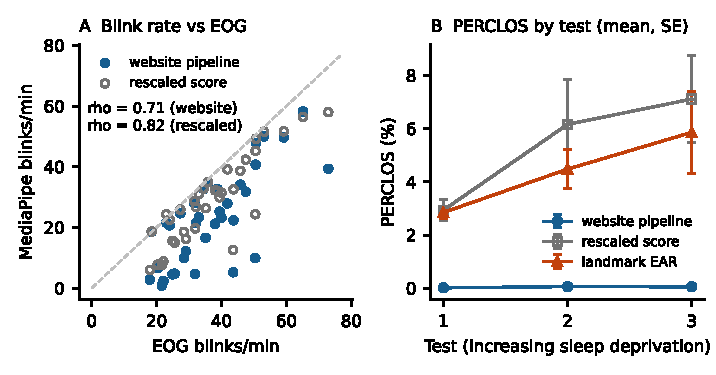
\includegraphics[width=\textwidth]{fig_drozy_mediapipe.pdf}
  \caption{The website's webcam pipeline (MediaPipe \texttt{eyeBlink} blendshapes and the unchanged blink meter) run on the 36 DROZY near-infrared videos. (A)~Blink rate against EOG blink rate, for the website pipeline and for a diagnostic per-test rescaling of the raw score. (B)~Mean PERCLOS by test (SE): the website pipeline stays near zero because the raw score rarely approaches 1. (C)~Mean blink duration from the website pipeline against KSS, one line per subject.}
  \label{fig:mediapipe}
\end{figure*}

\subsection{Replay of the released model on DROZY}
\label{sec:replay}
\paragraph*{Design} For each subject in turn, the forward models were refitted on the other 13 subjects. The model then replayed that subject's real test times, PVT median reaction times and per-minute webcam features (from the landmark pipeline), with or without the KSS rating of the first test as a check-in, and predicted the KSS of each later test from the events before it. DROZY does not record wake time, so we assumed waking at 07:00 after 7.5~h on the day of the first test, with 06:00 and 08:00 as sensitivity analyses. Each rating was placed 11~min after the start of its test. Confidence intervals come from 2000 bootstrap resamples of subjects. Conditions with a check-in need the first test, so they have 20 predictions from 10 subjects, against 24 from 12 subjects without.

\paragraph*{Results} The mean absolute error (MAE) was 1.73 KSS points for the prior alone, 1.51 for the PVT alone, 1.47 for the PVT and webcam, 1.51 for the check-in alone, 1.46 for the check-in and PVT, and 1.38 for all three (Fig.~\ref{fig:replay}). The prior over-predicted sleepiness on average (mean error $+0.81$), mostly at the night test (MAE 2.27 at test~2 against 1.18 at test~3); with all sources the mean error fell to $+0.31$ and the test-2 MAE to 1.60. Results were stable to the assumed wake time (all sources: 1.39 at 06:00 and 1.37 at 08:00; prior: 1.75 and 1.71). With two check-ins, predicting the third test (9 subjects), check-ins alone gave 1.90 and all sources 1.78; both under-predicted the final rating.

These results are indicative only. The intervals overlap widely, conditions with and without a check-in differ in their predictions, and two naive baselines bracket the model: carrying the first rating forward gave 3.45, but predicting each test by the mean rating of that test in the other subjects gave 1.39. That baseline knows the protocol, which a person's daily life does not provide, but it shows that the prior's time course, in particular its night-time level, is the largest source of error here.

\begin{figure}[t]
  \centering
  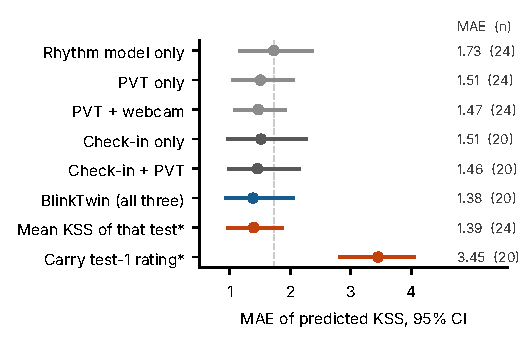
\includegraphics[width=\columnwidth]{fig_drozy_twin.pdf}
  \caption{Leave-one-subject-out replay of the released model on DROZY: MAE of predicted KSS for tests 2 and 3 (95\% CI over subjects; n = predictions). The check-in is the rating at test~1. *Naive baselines; the first uses the protocol's average course.}
  \label{fig:replay}
\end{figure}

\subsection{OpenNeuro ds004902}
\label{sec:openneuro}
\paragraph*{Data} The dataset contains 71 adults tested once after normal sleep and once after a night of sleep deprivation, in counterbalanced order~\cite{xiang2024resting,xiang2024ds004902}. We used only the participant table (version 1.0.4). KSS and SSS were collected in different participants, and only 2 people have both KSS and PVT data in both sessions.

\paragraph*{Group effects and a labelling discrepancy} After sleep deprivation, KSS rose by 2.03 points ($n = 33$, $d_z = 1.00$), the SSS by 1.66 ($n = 35$, $d_z = 0.80$) and the PVT median reaction time by 41.2~ms ($n = 30$, $d_z = 1.33$), while the number of lapses did not change ($p = 0.92$). KSS rose in 73\% of people, stayed the same in 18\% and fell in 9\%. Our paired $t$ statistics for the three PVT columns ($0.04$, $7.31$ and $4.72$ in absolute value for lapses, median and SD of reaction time) equal those in the dataset descriptor, but the descriptor attaches them to different measures. The released data dictionary and the value ranges (0--8 for lapses, 256--423~ms for median reaction time) support our assignment. Across the 25 people with PVT and SSS in both sessions, the change in reaction time was weakly related to the change in SSS (Spearman $\rho = 0.25$, approximate 95\% CI $-0.17$ to $0.59$).

\paragraph*{Does a person's offset persist?} Anchoring assumes that a person's offset from the prior is stable enough to be worth learning. For the 33 people with KSS in both sessions, we computed each person's offset from the prior in each session (default sleep assumption; KSS time taken as the eyes-open EEG time). The offsets were weakly correlated between sessions ($r = 0.29$, 95\% CI $-0.05$ to $0.58$; Spearman $0.32$). Predicting the rating after sleep deprivation, the prior alone gave an MAE of 1.53, the prior plus the person's shrunk offset from the other session 1.52, the full offset 1.63, and carrying the rating forward 2.33. An offset learned on one day therefore carries little information to a day weeks later. This agrees with the model's offset drift: with $\sqrt{q_d} = 0.3$ KSS~h$^{-1/2}$, the variance of the offset after 24~h without check-ins exceeds its prior variance, so a check-in's information is largely gone within a day.

\paragraph*{Can the prior be improved?} We fixed two comparisons in advance and report both. First, replacing the default sleep assumption with each person's sleep diary for the normal-sleep night (28 people) did not reduce the prior's MAE over the two sessions (1.74 against 1.69; difference $+0.06$, 95\% CI $-0.07$ to $+0.17$). Second, replacing the KSS mapping $10.6 - 0.6A$ with the mapping refitted to airline data by Ingre et al.~\cite{ingre2014validating}, $9.68 - 0.46A$, reduced it from 1.69 to 1.46 (difference $-0.22$, 95\% CI $-0.33$ to $-0.09$). The default mapping predicted a mean rise of 2.90 points after sleep deprivation and the refitted one 2.23, against an observed 2.04. With one check-in from the other session, the advantage of the refitted mapping shrank to $-0.09$ (95\% CI $-0.26$ to $+0.08$; all 33 people). Together with the prior's over-prediction at night in DROZY, this suggests that the default mapping is too steep for these samples. We have not changed the released default, because that requires re-running the DROZY replay; it is the first change to test.

\section{Simulation study}
\label{sec:simulation}

A simulation with a known ground truth answers questions that a short field study cannot: how much each source of information contributes, whether passive signals can be added safely, and how reliable the forecast is. The simulator (\texttt{web/src/sim/synth.ts}) and the evaluation (\texttt{web/scripts/simulate.ts}) call the same twin code as the website.

\subsection{Design}
\paragraph{Virtual participants.} Each virtual participant has a true sleepiness trajectory
\begin{equation}
  s^{*}(t) = \min\!\big(9, \max(1,\; p_{\phi}(t) + o + \gamma^{*} T(t) + \varepsilon(t))\big),
\end{equation}
where $p_{\phi}$ is the Three-Process Model prior with the person's circadian phase shifted by $\phi$, $o$ is a stable personal offset, $\gamma^{*}$ the person's time-on-task sensitivity and $\varepsilon$ a slow fluctuation (an Ornstein--Uhlenbeck process). Signals are generated from $s^{*}$ through person-specific mappings whose population distributions were taken from DROZY (Table~\ref{tab:population}): the PVT median reaction time is $r_0 + r_1(s^{*} - 3)$ plus noise, the mean blink duration is $b_0 + b_1(s^{*} - 3)$ plus noise, and PERCLOS is $\pi_0 + \pi_1 \max(0, s^{*} - 4)$ plus noise. KSS ratings are $s^{*}$ plus rating noise, rounded to integers and clipped to 1--9.

\paragraph{Cohorts.} Three disjoint cohorts with fixed random seeds were used. A \emph{training} cohort of 200 virtual people was used only to fit the population mappings, by ordinary least squares of KSS on each channel's features; the prior SDs of the weights were set to the between-person spread of per-person fits, with the per-person estimation noise removed by the method of moments. A \emph{tuning} cohort of 120 was used only to choose the webcam noise inflation $\kappa$, over a grid from 1 to 1280 and with the webcam switched off, at three check-ins. A \emph{test} cohort of 300 provides all reported results.

\paragraph{Protocol.} Each person wakes at 07:00 after 7.5~h of sleep and stays awake for 24~h, which spans the range from alert to very sleepy. The day alternates 50-minute task blocks with 10-minute breaks; the webcam yields one window per minute during task blocks; a reaction test is taken every 2~h and before each check-in. The number of KSS check-ins $k$ is 0, 1, 2, 3, 4, 6 or 8, spread evenly over the first 16~h.

\paragraph{Variants.} Six variants of the twin were compared, all on identical event streams:
\begin{enumerate}[label=(\Alph*),leftmargin=*,itemsep=1pt]
  \item \emph{Rhythm model only}: the Three-Process Model with the time-on-task term, no measurements.
  \item \emph{Check-ins only}: prior and KSS check-ins.
  \item \emph{Passive only}: prior, reaction tests and webcam through the population mappings, no check-ins, no bias states.
  \item \emph{Check-ins and passive, without anchoring}: as BlinkTwin but with both bias states fixed at zero.
  \item \emph{BlinkTwin}: check-ins anchor passive signals through the per-channel bias states (the default).
  \item \emph{BlinkTwin with personal slopes}: as (E), with the optional slope learning switched on.
\end{enumerate}

\paragraph{Outcomes.} The primary outcome is the mean absolute error (MAE) between the twin's estimate and the true latent sleepiness $s^{*}$, evaluated every 10 minutes from 30 minutes after waking to the end of the 24~h, averaged within each person and then across people, with 95\% bootstrap confidence intervals over people (1000 resamples). Paired differences between variants were computed per person and bootstrapped in the same way. Secondary outcomes were the coverage of the nominal 90\% intervals; and, for the event KSS $\geq$ 7 one hour ahead, the Brier score and the area under the ROC curve (AUROC), using forecasts made every hour from 12:00 to 05:00 with four check-ins (300 people $\times$ 18 forecasts = 5400; 20.5\% of outcomes were KSS $\geq$ 7).

\begin{table}[t]
  \centering
  \caption{Population distribution of virtual participants. Reaction-time, blink-duration and PERCLOS parameters were taken from DROZY.}
  \label{tab:population}
  \small
  \begin{tabular}{@{}lL{5.8cm}L{7.4cm}@{}}
    \toprule
    Parameter & Distribution & Meaning \\
    \midrule
    $o$ & $\mathcal{N}(0, 1.0)$ & Personal offset from the prior (KSS points) \\
    $\phi$ & $\mathcal{N}(0, 1.0)$ h & Circadian phase shift \\
    $\gamma^{*}$ & $\mathcal{N}(0.4, 0.2)$, $\geq 0$ & Time-on-task sensitivity (KSS h$^{-1}$) \\
    $\varepsilon$ & SD 0.5, time constant 1.5 h & Slow fluctuation of sleepiness \\
    Rating noise & SD 0.7, rounded & KSS check-in noise \\
    $r_0$, $r_1$ & $\mathcal{N}(339.2, 50.6)$ ms; $\mathcal{N}(18.8, 7.7)$ ms, $\geq 0$ & Reaction time at KSS 3; slope per KSS point (noise SD 36.1 ms) \\
    $b_0$, $b_1$ & $\mathcal{N}(187.5, 25.9)$ ms; $\mathcal{N}(11.9, 4.8)$ ms, $\geq 0$ & Blink duration at KSS 3; slope per KSS point (noise SD 43.1 ms) \\
    $\pi_0$, $\pi_1$ & 0.030; $\mathcal{N}(0.009, 0.005)$, $\geq 0$ & PERCLOS baseline; slope per KSS point above 4 (noise SD 0.023) \\
    Blink rate & $\mathcal{N}(17, 5)$ min$^{-1}$, $-0.12$ per TLX point & Baseline and load effect (noise SD 3) \\
    Workload & offset $\mathcal{N}(0, 10)$, fluctuation SD 6 & Around context demand; TLX noise SD 8 \\
    \bottomrule
  \end{tabular}
\end{table}

\subsection{Results}

\begin{table}[t]
  \centering
  \caption{Simulation: mean absolute error of the latent KSS estimate over 24~h (300 test participants), by variant and number of check-ins $k$, and coverage of the nominal 90\% intervals. Error is not strictly monotonic in $k$ because the check-in times change with $k$.}
  \label{tab:sim}
  \small
  \begin{tabular}{@{}L{5.1cm}cccccccc@{}}
    \toprule
    & \multicolumn{7}{c}{MAE by number of check-ins $k$} & Coverage \\
    \cmidrule(lr){2-8}
    Variant & 0 & 1 & 2 & 3 & 4 & 6 & 8 & ($k$ = 1) \\
    \midrule
    (A) Rhythm model only & 0.930 & & & & & & & 0.972$^{a}$ \\
    (B) Check-ins only & & 0.732 & 0.704 & 0.645 & 0.651 & 0.575 & 0.563 & 0.947 \\
    (C) Passive only & 0.837 & & & & & & & 0.832$^{a}$ \\
    (D) Check-ins + passive, no anchoring & & 0.740 & 0.699 & 0.649 & 0.656 & 0.587 & 0.573 & 0.853 \\
    (E) \textbf{BlinkTwin} (anchoring) & 0.843 & \textbf{0.703} & \textbf{0.674} & \textbf{0.625} & \textbf{0.640} & \textbf{0.572} & \textbf{0.558} & 0.913 \\
    (F) BlinkTwin + personal slopes & & 0.735 & 0.690 & 0.657 & 0.670 & 0.610 & 0.599 & 0.898 \\
    \bottomrule
    \multicolumn{9}{@{}l}{\footnotesize $^{a}$ At $k$ = 0.}
  \end{tabular}
\end{table}

\paragraph{Check-ins carry most of the information.} The rhythm model alone had an MAE of 0.930 KSS points (95\% CI 0.873 to 0.992). One check-in reduced this to 0.732, three to 0.645 and eight to 0.563 (Table~\ref{tab:sim}, Figure~\ref{fig:sim}A). Three check-ins in the first 16~h cut the error by about 31\% (paired difference $-0.285$, 95\% CI $-0.343$ to $-0.224$; BlinkTwin with three check-ins: $-0.305$, $-0.360$ to $-0.245$).

\paragraph{Passive signals help a little on their own.} With no check-ins, passive signals through the population mappings reduced the error from 0.930 to 0.837 (difference $-0.093$, 95\% CI $-0.133$ to $-0.054$), and BlinkTwin's anchored version to 0.843 ($-0.087$, $-0.117$ to $-0.054$). But without anchoring their 90\% intervals covered the truth only 83\% of the time, against 91\% for BlinkTwin.

\paragraph{Naive fusion does not help; anchoring does, a little, and safely.} Adding passive signals to one check-in without bias states gave no gain over the check-in alone (difference $+0.008$, 95\% CI $-0.022$ to $+0.038$) and lost calibration (coverage 0.853 against 0.947). With anchoring, the same signals reduced the error below check-ins alone (at $k$ = 1: $-0.029$, $-0.049$ to $-0.008$; at $k$ = 3: $-0.020$, $-0.034$ to $-0.007$) and below the unanchored fusion ($-0.037$, $-0.052$ to $-0.023$ at $k$ = 1), with coverage close to nominal (0.913). The gain fades as check-ins become frequent ($k$ = 8: $-0.005$, $-0.014$ to $+0.006$). Across all values of $k$, BlinkTwin was never worse than check-ins alone. The gains from passive signals over check-ins are small; the main value of anchoring is that passive signals can be added without making the estimate worse or overconfident.

\paragraph{Personal slopes hurt.} Learning each person's slopes from paired check-ins increased the error at every $k$ (at $k$ = 8: $+0.040$, 95\% CI $+0.034$ to $+0.046$; better for only 23\% of people), because a few noisy pairs move the slopes more than they inform them. The option is therefore off by default.

\paragraph{The webcam adds little to sleepiness estimation.} On the tuning cohort, treating each webcam minute as an independent observation ($\kappa$ = 1) made estimates worse (MAE 0.764 at $k$ = 3). The error fell as each minute was down-weighted, reached a minimum of 0.622 at $\kappa$ = 160, and rose slightly to 0.634 with the webcam switched off (Figure~\ref{fig:sim}B). The webcam therefore helps only slightly; its main role in BlinkTwin is the real-time alarm path, which this simulation does not evaluate.

\paragraph{Forecasts.} For KSS $\geq$ 7 one hour ahead, the Brier score was 0.098 for the rhythm model, 0.067 for check-ins only, 0.065 without anchoring, 0.062 for BlinkTwin and 0.065 with personal slopes, against 0.163 for a constant forecast of the base rate. The AUROC was 0.923, 0.964, 0.962, 0.964 and 0.961 respectively. BlinkTwin had the lowest Brier score, with the same discrimination as check-ins alone.

\begin{figure}[t]
  \centering
  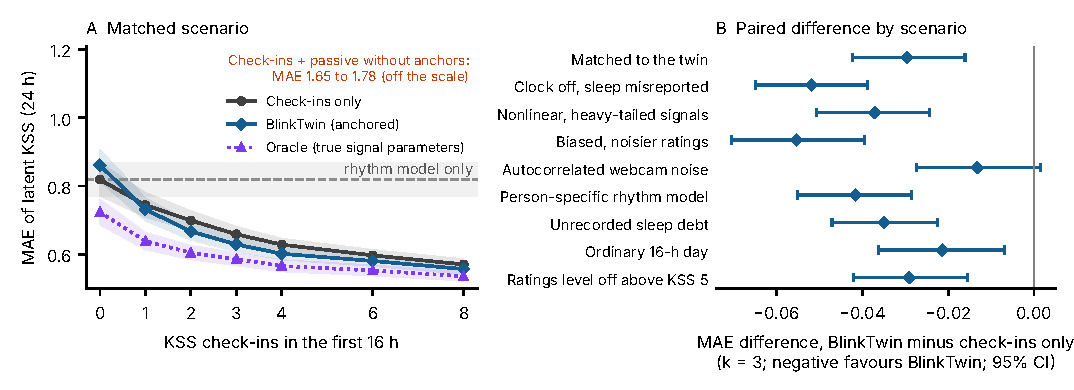
\includegraphics[width=\linewidth]{../results/fig_sim_mae.pdf}
  \caption{Simulation. (A) Mean absolute error of the latent KSS estimate over 24~h against the number of check-ins in the first 16~h, with 95\% bootstrap intervals (300 test participants). Horizontal lines: rhythm model only, and passive signals only. (B) Choice of the webcam noise inflation $\kappa$ on the separate tuning cohort (120 participants, three check-ins); ``off'' is the twin without the webcam.}
  \label{fig:sim}
\end{figure}

\section{Planned Validation Study}
\label{sec:protocol}

The analyses above use public laboratory data and simulation. Whether the approach helps real people in daily life needs a prospective study. We describe the planned design here; before any data are collected it will be registered on OSF Registries with a full statistical analysis plan, under an institutional sponsor and with approval from a human research ethics committee, and only then will it be pre-specified.

\paragraph*{Intended use and population} BlinkTwin is intended for self-monitoring by adults during desk work at a laptop. The study recruits adults aged 18--60 who work at a laptop for at least 4~h a day. Exclusions: night-shift work or transmeridian travel within two weeks; diagnosed sleep disorders; a positive screen for obstructive sleep apnoea (STOP-Bang~\cite{chung2008stop}); excessive daytime sleepiness (Epworth Sleepiness Scale above 10~\cite{johns1991new}); clinically relevant insomnia (Insomnia Severity Index of 15 or more~\cite{bastien2001validation}); pregnancy; and medication that affects alertness. Chronotype is measured with the Morningness--Eveningness Questionnaire~\cite{horne1976self}. Claims will be limited to this population.

\paragraph*{Field phase} Each participant uses BlinkTwin on their own computer for 10 working days in \emph{study mode}, which records events but hides every estimate, forecast, check and suggestion, so that the display cannot anchor ratings or change behaviour. Wrist actigraphy and a sleep diary record sleep; caffeine, alcohol and naps are logged. On each day the participant runs the webcam during laptop work and completes four check-ins at fixed times (09:30, 12:00, 14:30 and 17:00) and two \emph{probe} ratings at random times between them. Probe ratings are withheld from the model and used only for scoring, so that predictions between check-ins, where passive signals can matter, are evaluated. At each check-in the participant rates the KSS first, then takes the 3-min PVT-B, then rates NASA-TLX for the work block just finished. Each device's display and input latency is measured once with a photodiode and a key-press robot, or, where that is not possible, with a browser timing test, and the camera's frame rate is stored with every minute. Participants are told that BlinkTwin must not be used to decide whether they are fit to drive. Bystanders who may appear on the webcam at work, and the employer where relevant, are informed and asked for consent; no video is stored in the field phase.

\paragraph*{Laboratory phase} A subset takes part in a supervised session of up to 26~h of continuous wakefulness after at least 7 days of a stable sleep schedule verified by actigraphy, with simultaneous EEG, EOG and video. During the session the camera records desk work (typing, reading, phone use), not only the PVT or resting EEG. Additional exclusions apply (epilepsy, bipolar disorder, cardiovascular disease), caffeine and alcohol are not allowed from 24~h before, a physician is on call, and participants are taken home by arranged transport. Long eye closures and microsleeps are scored from EEG, EOG and video by two blinded raters using the BERN criteria~\cite{hertig2020microsleep}, and inter-rater agreement is reported. The number of participants is set by events, not by people: recruitment continues until at least 100 scored long eye closures are observed, which gives a 95\% confidence interval half-width of about 0.1 for a sensitivity near 0.7; analysis is per event with clustering by participant. Identifiable video is stored encrypted on institutional servers, used only for scoring and deleted after the study.

\paragraph*{Outcomes} Two co-primary outcomes: (1) the absolute error of predicting each probe rating, made from all earlier events (leave-future-out replay of the full 10-day log), with rating noise included in the interval; and (2) the absolute error of predicting the median reaction time of the next PVT-B, an objective outcome. Secondary outcomes: the error of predicting check-in ratings; coverage of the 90\% prediction interval, the probability integral transform and the continuous ranked probability score; the Brier score and AUROC for KSS $\geq 7$ within the next hour, in the laboratory phase where such ratings are common; sensitivity and positive predictive value of the alerts against scored events (laboratory) and alerts per hour with participant-labelled false alarms (field); agreement of the camera's blink measures with EOG; the false-flag rate of the reactions-versus-ratings check; the error of the predicted next TLX rating (exploratory); usability (System Usability Scale~\cite{brooke1996sus}); and adherence.

\paragraph*{Hypotheses and analysis} Methods are those of Section~\ref{sec:simulation}: the prior alone, check-ins only, the consider-covariance comparator and BlinkTwin. H1: on probe ratings, BlinkTwin is not worse than check-ins only, with a non-inferiority margin of 0.05 KSS points on the per-person mean absolute error (31\% of the simulated benefit of check-ins over the prior, 0.16 points), tested with a one-sided 97.5\% confidence bound and reported following the CONSORT extension for non-inferiority~\cite{piaggio2012reporting}. H2: on probe ratings, BlinkTwin is better than check-ins only, which is the test of the passive signals. H3: BlinkTwin predicts the next PVT-B better than the prior alone. H1 is tested first; H2 and H3 are tested at a Bonferroni-corrected $\alpha$ of 0.025 each. Absolute errors are also analysed with linear mixed models with method as a fixed effect and random intercepts for participant and day, as a sensitivity analysis. No parameter is tuned on the study data.

\paragraph*{Sample size} We estimated power by simulating the analysis that will be run, for check-in ratings: 1000 virtual people (the workday population of Section~\ref{sec:simulation}) each had 10 workdays replayed as one continuous event log, so that the offset and anchors carried over between days, with four check-ins a day each followed by a PVT-B; the prediction of each observed, noisy and rounded rating used all earlier events; and studies of $n$ people were drawn from the pool 5000 times. The mean error was 1.01 for the prior alone, 0.85 for check-ins only and 0.84 for BlinkTwin; per person, BlinkTwin minus check-ins averaged $-0.010$ (SD 0.036) and BlinkTwin minus the consider-covariance comparator $-0.014$ (SD 0.031). With a mean-reverting offset the difference from check-ins grew to $-0.028$ (24-h time constant) and $-0.047$ (72~h). Replaying each day separately instead, as in our earlier analysis, reversed the sign ($+0.019$), because the anchors were then relearnt every morning. Non-inferiority at a 0.05 margin had power above 0.99 from 20 people. Superiority of BlinkTwin over check-ins only had power 0.41 with 40, 0.68 with 80, 0.76 with 100 and 0.93 with 150 people (two-sided $\alpha = 0.05$). The co-primary outcomes on probe ratings and the next PVT-B, and the Bonferroni-corrected $\alpha$, have not yet been simulated; they will be before registration. Provisionally we plan to analyse 120 participants and to recruit 135. The generator keeps each person's offset constant across days, which the weak persistence in ds004902 contradicts, so these figures are likely optimistic for BlinkTwin.

\section{Discussion}
\label{sec:discussion}

\subsection{Principal findings}
On DROZY, point estimates of the error were lower with each added source (MAE 1.73 for the prior alone, 1.38 with a check-in and passive signals), but the intervals overlap, the prediction sets differ, the sample is small, and a protocol-aware naive baseline did as well. All of the gain arose at the night test, where the prior was most biased, and part of it is likely calibration transfer within one laboratory. On ds004902, a group-mean offset predicted ratings better than a person's own offset from another session, and the KSS mapping refitted by Ingre et al.~\cite{ingre2014validating} reduced the prior's error by 0.22 points, although DROZY's error lies in the prior's time course rather than its mapping. The website's camera pipeline, run on DROZY's near-infrared video, correlated with EOG blink rate but undercounted blinks by about a third; its blink-duration association with sleepiness was confounded with frame rate; and its PERCLOS failed, so the model now ignores PERCLOS in that case. In simulation, check-ins carried most of the information, and passive signals alone did not improve on the prior. Estimating per-signal anchors gave a small gain (0.03 KSS points over check-ins only, 0.04 over a filter that allows for persistent biases without estimating them), which held when the model's assumptions were broken. In a simulation of the planned 10-day study, replayed as one continuous log, passive signals improved the prediction of observed ratings by 0.01 points, and a mean-reverting offset by a further 0.02 to 0.04; when each day was replayed separately, so that the anchors were relearnt every morning, the passive signals made predictions slightly worse. The value of the anchors therefore depends on carrying them across days. The evidence supports check-ins as the main source of information and anchored passive signals as a small addition whose value in real use is unproven.

\subsection{Comparison with other work}
Table~\ref{tab:comparison} lists published results for related problems. No study we found reports KSS regression error on DROZY or ds004902; published DROZY results are binary classifications~\cite{maior2020realtime}, which cannot be compared with an MAE, so our numbers are a first reference point on these datasets rather than evidence that BlinkTwin is more accurate than other systems. On the KSS scale, our errors are in the range expected for the Three-Process Model: Ingre et al.\ reported an in-sample residual SD of 1.46 in field data~\cite{ingre2014validating}, and Knock et al.\ predicted 48--60\% of shift workers' ratings within one point~\cite{knock2021prediction}, against 36\% for our prior on ds004902 (45\% with the refitted mapping). The closest designs predict PVT performance rather than self-rated sleepiness. Subramaniyan et al.\ fed face-video features into a personalised model and reached an error close to the PVT's own within-person variability~\cite{subramaniyan2025personalized}, the 2B-Alert app needed about 12 PVTs to reach its best accuracy~\cite{reifman2019twobalert}, and Ahlstrom et al.\ improved a sleep/wake predictor's forecast of high KSS with an eye-movement test~\cite{ahlstrom2013fit}. That personal learning needs many observations is consistent with our finding that one or two check-ins help little. Accuracy on real drowsiness from consumer cameras is modest: on UTA-RLDD the best video model reached 65.2\% on three classes and human judges 57.8\%~\cite{ghoddoosian2019realistic}.

\subsection{Subjective and objective sleepiness}
Anchoring makes the person's ratings the reference, which is right for an estimate of how sleepy a person feels but can hide objective decline~\cite{vandongen2003cumulative,leproult2003individual}. A single reaction test read on the population scale cannot reveal that decline, because people's baselines differ by about 2.6 KSS-equivalents and device latency shifts the level. The application therefore flags a possible dissociation only from within-person change in the reaction-time anchor, and presents the check as experimental. Its false-alarm rate, detection delay and effect on behaviour are untested; a chronic-restriction scenario, in which ratings level off over days while performance declines, is the right test.

\subsection{How accuracy could improve}
In order of the evidence we have: (i)~a mean-reverting offset, which lowered simulated error without loss of coverage in the one-day study, improved rating prediction most in the 10-day power simulation, and matches the weak persistence in ds004902; (ii)~a personal state beyond an additive offset, such as a gain on homeostatic pressure or a circadian phase shift, which trait-like vulnerability~\cite{vandongen2004systematic} predicts and which two sessions at different sleep pressure can identify; (iii)~the field-refitted KSS mapping, supported by ds004902 but not by DROZY; (iv)~forward models refitted on the website's own camera features, with the closed-eye level normalised to the person, the blink-duration noise inflation matched to that pipeline, long closures as a further signal, and the frame rate, which the application now stores with every minute, used to exclude or model low-rate minutes; (v)~a lapse- or speed-based PVT model fitted on the PVT-B itself; and (vi)~check-ins scheduled where they are most informative, which the application now suggests.

\subsection{Limitations}
The real-data evaluation rests on 14 people in DROZY and 33 in ds004902, with near-infrared rather than RGB video, a 10-min rather than 3-min PVT, assumed wake times in DROZY, frame rate confounded with sleep deprivation, and landmark rather than MediaPipe features in the replay. The forward-model slopes are fitted on noisy, integer ratings and are therefore attenuated~\cite{carroll2006measurement}, and slope heterogeneity is treated as independent noise although it is a persistent person-level error. The EOG reference was an automatic detector without manual annotation, and event-level blink and long-closure accuracy was not measured. Browser reaction times include device latency that we have not yet measured. The KSS is treated as a continuous Gaussian measurement although it is an integer scale with a ceiling, and the model's interval describes the latent state, not a future rating, unless rating noise is added. The prior uses local clock time without phase adaptation, so travel, shift work and daylight-saving changes produce time-varying errors that the offset cannot absorb. The time-on-task term, the offset's dynamics and the alert thresholds are assumptions, and the forward-pitch sign of the head-drop alert has not been verified on devices. The simulation, although it includes misspecified scenarios and a fair comparator, is built from the model's own structure, and the 24-h scenario lies outside the intended use; on an ordinary workday sleepiness of KSS~7 or more was rare. The privacy check used a test pattern without a face. Workload was not evaluated. BlinkTwin is not a medical device.

\subsection{Ethics and privacy}
Webcam monitoring at work raises concerns about surveillance. BlinkTwin is designed for self-monitoring: frames never leave the page, a content security policy blocks all connections other than to the site and the model host, only one-minute numeric summaries are stored in the person's browser (unencrypted, which matters on shared computers), and the person can export or delete them. Any deployment by an employer would need informed consent, transparency about what is measured, and a guarantee that the data are not used against the person.

\section{Conclusion}
\label{sec:conclusion}
BlinkTwin estimates how sleepy a person feels by joining the published Three-Process Model with occasional KSS check-ins and with reaction-time and camera signals that each have their own personal anchor, entirely in a browser and with video kept on the device. On public data, check-ins and the prior's time course mattered most, the camera pipeline measured blinks but not PERCLOS on near-infrared video, and the passive signals' benefit was small and confined to simulation. Validation of the camera pipeline on ordinary webcams and the planned prospective study are needed before any claim about daily use.

\section*{Data and Code Availability}
\label{sec:statements}
The source code of BlinkTwin, the analysis scripts, the simulation code, the result files and the scripts that produce every figure are at \url{https://github.com/r11up/BlinkTwin}. A versioned snapshot will be archived with a DOI on submission, and the commit used for this manuscript will be stated. The TypeScript scripts run directly in Node.js 22.6 or later (type stripping); the Python analyses use Python 3.13 with pinned packages. OpenNeuro ds004902 is openly available~\cite{xiang2024ds004902}. DROZY is available from the University of Li\`ege under a research-only licence that does not permit redistribution~\cite{massoz2016ulg}; it is not included, a script downloads it for users who accept its terms, and only aggregate results derived from it are reported or stored in the repository.

\section*{Acknowledgment}
The author thanks the creators of DROZY and OpenNeuro ds004902 for making their data available. The author declares no competing interests. This work received no specific funding.


\bibliographystyle{IEEEtran}
\bibliography{refs}

\end{document}
